\documentclass[10pt, a4paper]{article}
\usepackage{a4wide}
\usepackage{amsmath}
\usepackage{amsfonts}
\usepackage{graphicx}
\usepackage{verbatim}
\usepackage{epstopdf}
\usepackage{makeidx}
\usepackage{xcolor}
\usepackage{listings}
\usepackage{moreverb}
\definecolor{gogetit}{HTML}{6C8B9F}
\definecolor{greencomments}{rgb}{0,0.5,0}

\usepackage{color}
\usepackage{listings}
\lstset{ %
language=C,                % choose the language of the code
basicstyle=\footnotesize,       % the size of the fonts that are used for the code
numbers=left,                   % where to put the line-numbers
numberstyle=\footnotesize,      % the size of the fonts that are used for the line-numbers
stepnumber=1,                   % the step between two line-numbers. If it is 1 each line will be numbered
numbersep=12pt,                  % how far the line-numbers are from the code
backgroundcolor=\color{white},  % choose the background color. You must add \usepackage{color}
commentstyle=\itshape\color{gogetit},
keywordstyle=\bfseries\color{greencomments},
stringstyle=\color{blue},
escapeinside={(*@}{@*)},
showspaces=false,               % show spaces adding particular underscores
showstringspaces=false,         % underline spaces within strings
showtabs=true,                 % show tabs within strings adding particular underscores
frame=single,           % adds a frame around the code
tabsize=2,          % sets default tabsize to 2 spaces
captionpos=b,           % sets the caption-position to bottom
breaklines=true,        % sets automatic line breaking
breakatwhitespace=false,    % sets if automatic breaks should only happen at whitespace
escapeinside={\%*}{*)}          % if you want to add a comment within your code
}
\usepackage{caption}
\DeclareCaptionFont{white}{\color{white}}
\DeclareCaptionFormat{listing}{\colorbox[cmyk]{0.43, 0.35, 0.35,0.01}{\parbox{\textwidth}{\hspace{15pt}#1#2#3}}}
\captionsetup[lstlisting]{format=listing,labelfont=white,textfont=white, singlelinecheck=false, margin=0pt, font={bf,footnotesize}}

\newcommand{\real}{\mathbb{R}}
\newcommand{\nat}{\mathbb{N}}
\newcommand{\eme}{\mathcal{M}}
\newcommand{\emeh}{\widehat{\mathcal{M}}}
\newcommand{\ere}{\mathcal{R}}
\newcommand{\cee}{\mathcal{C}}


\usepackage{caratulaMetNum}
\materia{Organizaci\'on del computador 2}
\titulo{Trabajo Pr\'actico N\'umero 2}
\integrante{Facundo B\'alsamo}{xxx/xx}{balsa@mo.com.ar}
\integrante{Pablo Gonz\'alez}{xxx/xx}{pablo@gonzalez.com.ar}
\integrante{Lasso, Nicol\'as}{763/10}{lasso.nico@gmail.com}

\abstracto{[Breve introduccion de no mas de 200 palabras]}

\palabraClave{palabraClave1}
\palabraClave{palabraClave2}
\palabraClave{palabraClave3}
\palabraClave{palabraClave4}

\makeindex
\renewcommand{\indexname}{Indice}
\begin{document}
\maketitle 

\index{Introducci\'on Teorica}
\section{Introducci\'on Te\'orica}
El siguiente trabajo pr\'actico tiene como finalidad el uso de la programaci\'on SIMD orientado al procesamiento de im\'agenes. Para ello se aplican filtros para procesar dichas im\'agenes mediante el uso tanto de lenguaje ensamblador como lenguaje C.\newline
\indent La finalidad de la implementaci\'on en dos lenguajes es medir la velocidad de ejecucion y cantidad de cilos que son necesarios al aplicar los filtros para cada uno y as\'i compararlos.
\index{Desarrollo|(}
\section{Desarrollo}

En esta secci\'on se explica detalladamente cada uno de los filtros \'utilizados para procesar las im\'agenes:

\subsection{Filtro de color:}

Este filtro consiste b\'asicamente en dados un color y una distancia o threshold pasados como par\'ametros, procesa cada pixel de una im\'agen a color evaluando si el color del mismo se "aleja" m\'as de la distancia del par\'ametro, y si eso pasa, el pixel se transforma a blanco y negro, sino lo mantiene igual.
\subsubsection{Implementaci\'on en C:}
\subsubsection{Implementaci\'on en asm}
\subsubsection{Resultados}

\subsection{Filtro miniature:}

Este filtro consiste en procesar una im\'agen y hacer que los objetos se vean pequeños o de juguetes. Para esto se "desenfoca" una parte superior y otra inferior de la im\'agen, y as\'i s\'olo queda el foco en la parte del medio, logrando dicho efecto.
\subsubsection{Implementaci\'on en C:}
\subsubsection{Implementaci\'on en asm}
\subsubsection{Resultados}

\subsection{Decodificaci\'on Esteganogr\'afica:}

\subsubsection{Implementaci\'on en C:}
\subsubsection{Implementaci\'on en asm}
\subsubsection{Resultados}
\index{Desarrollo|)}
\index{Resultado|(}
\section{Resultado}
\subsection{Resultados de experimentaci\'on con diferentes n}
\begin{itemize}
\item
  \begin{itemize}
    \item Parametros de entrada:
	  \begin{itemize}
	    \item Span: 18
	    \item h: 1
	    \item n: 4
	    \item $c_i$: 0.5
	    \item Costo Unitario: 2000
	    \item FMax: 10
	  \end{itemize}
      \item Resultados:
	  \begin{itemize}
	    \item Costo Final: 2000
	    \item Pilares insertados: 0
	    \item Fuerza Maxima ejercida: F7 4
	  \end{itemize}
      \end{itemize} 
\item 
    \begin{itemize}
    \item Parametros de entrada:
	  \begin{itemize}
	    \item Span: 18
	    \item h: 1
	    \item n: 6
	    \item $c_i$: 0.5
	    \item Costo Unitario: 2000
	    \item FMax: 10
	  \end{itemize}
      \item Resultados:
	  \begin{itemize}
	    \item Costo Final: 2000
	    \item Pilares insertados: 0. No fue necesario.
	    \item Fuerza Maxima ejercida subpuente 1: F11 6.75
	  \end{itemize}
      \end{itemize}
\item
  \begin{itemize}
    \item Parametros de entrada:
	  \begin{itemize}
	    \item Span: 18
	    \item h: 1
	    \item n: 8
	    \item $c_1$: 0.5
	    \item $c_2$: 0.5
	    \item $c_3$: 0.5
	    \item $c_4$: 0.5
	    \item $c_5$: 0.5
	    \item Costo Unitario: 2000
	    \item FMax: 10
	  \end{itemize}
      \item Resultados:
	  \begin{itemize}
	    \item Costo Final: 2000
	    \item Pilares insertados: 0
	    \item Fuerza Maxima ejercida: F15 8
	  \end{itemize}
      \end{itemize}

\item
  \begin{itemize}
    \item Parametros de entrada:
	  \begin{itemize}
	    \item Span: 100
	    \item h: 1
	    \item n: 90
	    \item $c_i$: 0.5
	    \item Costo Unitario: 2000
	    \item FMax: 20
	  \end{itemize}
      \item Resultados:
	  \begin{itemize}
	    \item Costo Final: 48841.5
	    \item Pilares insertados: 7
	    \item Fuerza Maxima ejercida en uno de los subpuentes fue: F23 9
	    \item Obs: Para el resto de la FM\'ax, estuvieron acotadas por 9.
	  \end{itemize}
      \end{itemize}
\item
  \begin{itemize}
    \item Parametros de entrada:
	  \begin{itemize}
	    \item Span: 100
	    \item h: 1
	    \item n: 80
	    \item $c_i$: 0.5
	    \item Costo Unitario: 2000
	    \item FMax: 20
	  \end{itemize}
      \item Resultados:
	  \begin{itemize}
	    \item Costo Final: 41423.8
	    \item Pilares insertados: 7
	    \item Fuerza Maxima ejercida en uno de los subpuentes fue: F19 12.5
	    \item Obs: Para el resto de la FM\'ax, estuvieron acotadas por 12.5.
	  \end{itemize}
      \end{itemize}
\item
  \begin{itemize}
    \item Parametros de entrada:
	  \begin{itemize}
	    \item Span: 100
	    \item h: 1
	    \item n: 70
	    \item $c_i$: 0.5
	    \item Costo Unitario: 2000
	    \item FMax: 20
	  \end{itemize}
      \item Resultados:
	  \begin{itemize}
	    \item Costo Final: 34924.3
	    \item Pilares insertados: 7
	    \item Fuerza Maxima ejercida en uno de los subpuentes fue: F19 18.75
	    \item Obs: Para el resto de la FM\'ax, estuvieron acotadas por 12.
	  \end{itemize}
      \end{itemize}
\item
  \begin{itemize}
    \item Parametros de entrada:
	  \begin{itemize}
	    \item Span: 100
	    \item h: 1
	    \item n: 50
	    \item $c_i$: 0.5
	    \item Costo Unitario: 2000
	    \item FMax: 20
	  \end{itemize}
      \item Resultados:
	  \begin{itemize}
	    \item Costo Final: 25267.3
	    \item Pilares insertados: 4
	    \item Fuerza Maxima ejercida en uno de los subpuentes fue: F15 8
	    \item Obs: Para el resto de la FM\'ax, estuvieron acotadas por 4.5.
	  \end{itemize}
      \end{itemize}
\item
  \begin{itemize}
    \item Parametros de entrada:
	  \begin{itemize}
	    \item Span: 100
	    \item h: 1
	    \item n: 40
	    \item $c_i$: 0.5
	    \item Costo Unitario: 2000
	    \item FMax: 20
	  \end{itemize}
      \item Resultados:
	  \begin{itemize}
	    \item Costo Final: 21307.2
	    \item Pilares insertados: 3
	    \item Fuerza Maxima ejercida en uno de los subpuentes fue: F19 18.75
	    \item Obs: Para el resto de la FM\'ax, estuvieron acotadas por 18.75.
	  \end{itemize}
      \end{itemize}
\item
  \begin{itemize}
    \item Parametros de entrada:
	  \begin{itemize}
	    \item Span: 100
	    \item h: 1
	    \item n: 10
	    \item $c_i$: 0.5
	    \item Costo Unitario: 2000
	    \item FMax: 20
	  \end{itemize}
      \item Resultados:
	  \begin{itemize}
	    \item Costo Final: 5818.29
	    \item Pilares insertados: 2
	    \item Fuerza Maxima ejercida el subpuente de la seccion 1: F7 10
	    \item Fuerza Maxima ejercida el subpuente de la seccion 2: F6 -5.07544
	    \item Fuerza Maxima ejercida el subpuente de la seccion 3: F7 10
	  \end{itemize}
      \end{itemize}	
\item
  \begin{itemize}
    \item Parametros de entrada:
	  \begin{itemize}
	    \item Span: 100
	    \item h: 1
	    \item n: 6
	    \item $c_i$: 0.5
	    \item Costo Unitario: 2000
	    \item FMax: 20
	  \end{itemize}
      \item Resultados:
	  \begin{itemize}
	    \item Costo Final: 2000
	    \item Pilares insertados: 1
	    \item Fuerza Maxima ejercida el subpuente de la seccion 1: F6 -9.04174
	    \item Fuerza Maxima ejercida el subpuente de la seccion 2: F7 17
	  \end{itemize}
      \end{itemize}
\end{itemize}
\subsection{Resultados de experimentaci\'on con diferentes Fuerzas M\'aximas}
\begin{itemize}
\item
  \begin{itemize}
    \item Parametros de entrada:
	  \begin{itemize}
	    \item Span: 18
	    \item h: 1
	    \item n: 6
	    \item $c_i$: 0.5
	    \item Costo Unitario: 2000
	    \item FMax: 5
	  \end{itemize}
      \item Resultados:
	  \begin{itemize}
	    \item Costo Final: 2000
	    \item Pilares insertados: 1
	    \item Fuerza Maxima ejercida en el subpuente 1 de 2 secciones: F6 -1.76744
	    \item Fuerza Maxima ejercida en el subpuente 2 de 4 secciones: F7 3
	  \end{itemize}
      \end{itemize}
\item
  \begin{itemize}
    \item Parametros de entrada:
	  \begin{itemize}
	    \item Span: 18
	    \item h: 1
	    \item n: 6
	    \item $c_i$: 0.5
	    \item Costo Unitario: 2000
	    \item FMax: 10
	  \end{itemize}
      \item Resultados:
	  \begin{itemize}
	    \item Costo Final: 2000
	    \item Pilares insertados: 0
	    \item Fuerza Maxima ejercida: F11 6.75
	  \end{itemize}
      \end{itemize}
\item
  \begin{itemize}
    \item Parametros de entrada:
	  \begin{itemize}
	    \item Span: 18
	    \item h: 1
	    \item n: 6
	    \item $c_i$: 0.5
	    \item Costo Unitario: 2000
	    \item FMax: 3
	  \end{itemize}
      \item Resultados:
	  \begin{itemize}
	    \item Costo Final: 2000
	    \item Pilares insertados: 1
	    \item Fuerza Maxima ejercida en el subpuente 1 de 2 secciones: F6 -1.76744
	    \item Fuerza Maxima ejercida en el subpuente 2 de 4 secciones: F7 3
	  \end{itemize}
      \end{itemize}
\item
  \begin{itemize}
    \item Parametros de entrada:
	  \begin{itemize}
	    \item Span: 18
	    \item h: 1
	    \item n: 6
	    \item $c_i$: 0.5
	    \item Costo Unitario: 2000
	    \item FMax: 2
	  \end{itemize}
      \item Resultados:
	  \begin{itemize}
	    \item Costo Final: 4235.54
	    \item Pilares insertados: 2
	    \item Fuerza Maxima ejercida en el subpuente 1 de 2 secciones: F6 -1.76744
	    \item Fuerza Maxima ejercida en el subpuente 2 de 2 secciones: F6 -1.76744
	    \item Fuerza Maxima ejercida en el subpuente 2 de 2 secciones: F6 -1.76744
	  \end{itemize}
      \end{itemize}
\item
  \begin{itemize}
    \item Parametros de entrada:
	  \begin{itemize}
	    \item Span: 18
	    \item h: 1
	    \item n: 6
	    \item $c_i$: 0.5
	    \item Costo Unitario: 2000
	    \item FMax: 1
	  \end{itemize}
      \item Resultados:
	  \begin{itemize}
	    \item Costo Final: 4235.54
	    \item Pilares insertados: 2
	    \item Fuerza Maxima ejercida en el subpuente 1 de 2 secciones: F6 -1.76744
	    \item Fuerza Maxima ejercida en el subpuente 2 de 2 secciones: F6 -1.76744
	    \item Fuerza Maxima ejercida en el subpuente 2 de 2 secciones: F6 -1.76744
	    \item Obs: En este caso result\'o extraño. Con fuerzas m\'aximas muy pequeñas no se puede construir el puente. habr\'ia que insertar un pilar
por cada secci\'on del mismo.
	  \end{itemize}
      \end{itemize}
\subsection{Resultados de experimentaci\'on con Span muy grande:}
\item
  \begin{itemize}
    \item Parametros de entrada:
	  \begin{itemize}
	    \item Span: 100
	    \item h: 1
	    \item n: 6
	    \item $c_i$: 0.5
	    \item Costo Unitario: 2000
	    \item FMax: 20
	  \end{itemize}
      \item Resultados:
	  \begin{itemize}
	    \item Costo Final: 2000
	    \item Pilares insertados: 1
	    \item Fuerza Maxima ejercida en el subpuente 1 de 2 secciones: F6 -9.04174
	    \item Fuerza Maxima ejercida en el subpuente 2 de 4 secciones: F7 17
	  \end{itemize}
      \end{itemize}
\item
  \begin{itemize}
    \item Parametros de entrada:
	  \begin{itemize}
	    \item Span: 100
	    \item h: 1
	    \item n: 100
	    \item $c_i$: 0.5
	    \item Costo Unitario: 2000
	    \item FMax: 20
	  \end{itemize}
      \item Resultados:
	  \begin{itemize}
	    \item Costo Final: 57106.7
	    \item Pilares insertados: 7
	    \item Fuerza Maxima ejercida en uno de los subpuentes fue: F27 12.25
	    \item Obs: Para el resto de la FM\'ax, estuvieron acotadas por 9.
	  \end{itemize}
      \end{itemize}
\item
  \begin{itemize}
    \item Parametros de entrada:
	  \begin{itemize}
	    \item Span: 100
	    \item h: 100
	    \item n: 100
	    \item $c_i$: 0.5
	    \item Costo Unitario: 2000
	    \item FMax: 20
	  \end{itemize}
      \item Resultados:
	  \begin{itemize}
	    \item Costo Final: 119083
	    \item Pilares insertados: 30
	    \item Fuerza Maxima ejercida en uno de los subpuentes fue: F3 19.0135
	    \item Obs: Para el resto de la FM\'ax, estuvieron acotadas por F2 -0.510308.
	  \end{itemize}
      \end{itemize}
\item
  \begin{itemize}
    \item Parametros de entrada:
	  \begin{itemize}
	    \item Span: 100
	    \item h: 50
	    \item n: 100
	    \item $c_i$: 0.5
	    \item Costo Unitario: 2000
	    \item FMax: 20
	  \end{itemize}
      \item Resultados:
	  \begin{itemize}
	    \item Costo Final: 89834.9
	    \item Pilares insertados: 30
	    \item Fuerza Maxima ejercida en uno de los subpuentes fue: F3 19.0163
	    \item Obs: Para el resto de la FM\'ax, estuvieron acotadas por F2 -0.510308.
	  \end{itemize}
      \end{itemize}
\item
  \begin{itemize}
    \item Parametros de entrada:
	  \begin{itemize}
	    \item Span: 100
	    \item h: 25
	    \item n: 100
	    \item $c_i$: 0.5
	    \item Costo Unitario: 2000
	    \item FMax: 20
	  \end{itemize}
      \item Resultados:
	  \begin{itemize}
	    \item Costo Final: 2000
	    \item Pilares insertados: 1
	    \item Fuerza Maxima ejercida en el subpuente 1 de 50 secciones: F198 12.2598
	    \item Fuerza Maxima ejercida en el subpuente 2 de 50 secciones: F198 12.2598
	  \end{itemize}
      \end{itemize}
\item
  \begin{itemize}
    \item Parametros de entrada:
	  \begin{itemize}
	    \item Span: 100
	    \item h: 5
	    \item n: 100
	    \item $c_i$: 0.5
	    \item Costo Unitario: 2000
	    \item FMax: 20
	  \end{itemize}
      \item Resultados:
	  \begin{itemize}
	    \item Costo Final: 124394
	    \item Pilares insertados: 3
	    \item Fuerza Maxima ejercida en uno de los subpuentes fue: F51 8.45
	    \item Obs: Para el resto de la FM\'ax, estuvieron acotadas por F47 7.2.
	  \end{itemize}
      \end{itemize}
\item
  \begin{itemize}
    \item Parametros de entrada:
	  \begin{itemize}
	    \item Span: 100
	    \item h: 8
	    \item n: 100
	    \item $c_i$: 0.5
	    \item Costo Unitario: 2000
	    \item FMax: 20
	  \end{itemize}
      \item Resultados:
	  \begin{itemize}
	    \item Costo Final: 2000
	    \item Pilares insertados: 1
	    \item Fuerza Maxima ejercida en el subpuente 1 de 50 secciones: F99 19.5312
	    \item Fuerza Maxima ejercida en el subpuente 2 de 50 secciones: F99 19.5312
	  \end{itemize}
      \end{itemize}
\item
  \begin{itemize}
    \item Parametros de entrada:
	  \begin{itemize}
	    \item Span: 100
	    \item h: 30
	    \item n: 100
	    \item $c_i$: 0.5
	    \item Costo Unitario: 2000
	    \item FMax: 20
	  \end{itemize}
      \item Resultados:
	  \begin{itemize}
	    \item Costo Final: 38136.9
	    \item Pilares insertados: 10
	    \item Fuerza Maxima ejercida en uno de los subpuentes fue: F3 19.761
	    \item Obs: Para el resto de la FM\'ax, estuvieron acotadas por F2 -0.517539.
	  \end{itemize}
      \end{itemize}
\item
  \begin{itemize}
    \item Parametros de entrada:
	  \begin{itemize}
	    \item Span: 100
	    \item h: 1
	    \item n: 100
	    \item $c_i$: 0.5
	    \item Costo Unitario: 2000
	    \item FMax: 50
	  \end{itemize}
      \item Resultados:
	  \begin{itemize}
	    \item Costo Final: 49106.7
	    \item Pilares insertados: 3
	    \item Fuerza Maxima ejercida en uno de los subpuentes fue: F51 42.25
	    \item Obs: Para el resto de la FM\'ax, estuvieron acotadas por F47 36.
	  \end{itemize}
      \end{itemize}
\item
  \begin{itemize}
    \item Parametros de entrada:
	  \begin{itemize}
	    \item Span: 100
	    \item h: 1
	    \item n: 100
	    \item $c_i$: 0.5
	    \item Costo Unitario: 2000
	    \item FMax: 200
	  \end{itemize}
      \item Resultados:
	  \begin{itemize}
	    \item Costo Final: 2000
	    \item Pilares insertados: 1
	    \item Fuerza Maxima ejercida en ambos subpuentes: F99 156.25
	  \end{itemize}
      \end{itemize}
\item
  \begin{itemize}
    \item Parametros de entrada:
	  \begin{itemize}
	    \item Span: 100
	    \item h: 1
	    \item n: 100
	    \item $c_i$: 0.5
	    \item Costo Unitario: 2000
	    \item FMax: 150
	  \end{itemize}
      \item Resultados:
	  \begin{itemize}
	    \item Costo Final: 49106.7
	    \item Pilares insertados: 3
	    \item Fuerza Maxima ejercida en uno de los subpuentes fue: F51 42.25
	    \item Obs: Para el resto de la FM\'ax, estuvieron acotadas por F47 36.
	  \end{itemize}
      \end{itemize}
\item
  \begin{itemize}
    \item Parametros de entrada:
	  \begin{itemize}
	    \item Span: 100
	    \item h: 1
	    \item n: 100
	    \item $c_i$: 0.5
	    \item Costo Unitario: 2000
	    \item FMax: 40
	  \end{itemize}
      \item Resultados:
	  \begin{itemize}
	    \item Costo Final: 53106.7
	    \item Pilares insertados: 5
	    \item Fuerza Maxima ejercida en uno de los subpuentes fue: F51 42.25
	    \item Obs: Para el resto de la FM\'ax, estuvieron acotadas por F47 36.
	  \end{itemize}
      \end{itemize}
\item
  \begin{itemize}
    \item Parametros de entrada:
	  \begin{itemize}
	    \item Span: 100
	    \item h: 1
	    \item n: 100
	    \item $c_i$: 0.5
	    \item Costo Unitario: 2000
	    \item FMax: 10
	  \end{itemize}
      \item Resultados:
	  \begin{itemize}
	    \item Costo Final: 61106.7
	    \item Pilares insertados: 9
	    \item Fuerza Maxima ejercida en uno de los subpuentes fue: F15 4
	    \item Obs: Para el resto de la FM\'ax, estuvieron acotadas por F11 2.25.
	  \end{itemize}
      \end{itemize}
\end{itemize}
\subsection{Resultados de experimentaci\'on con diferentes Fuerzas C}
\begin{itemize}
\item
  \begin{itemize}
    \item Parametros de entrada:
	  \begin{itemize}
	    \item Span: 100
	    \item h: 1
	    \item n: 100
	    \item $c_i$: 1
	    \item Costo Unitario: 2000
	    \item FMax: 20
	  \end{itemize}
      \item Resultados:
	  \begin{itemize}
	    \item Costo Final: 61106.7
	    \item Pilares insertados: 9
	    \item Fuerza Maxima ejercida en uno de los subpuentes fue: F15 8
	    \item Obs: Para el resto de la FM\'ax, estuvieron acotadas por F11 4.5.
	  \end{itemize}
      \end{itemize}
\item
  \begin{itemize}
    \item Parametros de entrada:
	  \begin{itemize}
	    \item Span: 100
	    \item h: 1
	    \item n: 100
	    \item $c_i$: 1.5
	    \item Costo Unitario: 2000
	    \item FMax: 20
	  \end{itemize}
      \item Resultados:
	  \begin{itemize}
	    \item Costo Final: 73106.7
	    \item Pilares insertados: 15
	    \item Fuerza Maxima ejercida en uno de los subpuentes fue: F15 12
	    \item Obs: Para el resto de la FM\'ax, estuvieron acotadas por F11 6.75.
	  \end{itemize}
      \end{itemize}
\item
  \begin{itemize}
    \item Parametros de entrada:
	  \begin{itemize}
	    \item Span: 100
	    \item h: 1
	    \item n: 100
	    \item $c_i$: 0.25
	    \item Costo Unitario: 2000
	    \item FMax: 20
	  \end{itemize}
      \item Resultados:
	  \begin{itemize}
	    \item Costo Final: 53106.7
	    \item Pilares insertados: 5
	    \item Fuerza Maxima ejercida en uno de los subpuentes fue: F27 6.125
	    \item Obs: Para el resto de la FM\'ax, estuvieron acotadas por F23 4.5.
	  \end{itemize}
      \end{itemize}
\end{itemize}

\subsection{Resultados de experimentaci\'on en funci\'on del span:}
\subsubsection{Parametros de entrada Fijos:}
los parametros que no var\'ian son:
  \begin{itemize}
      \item h: 1
      \item n: 6
      \item $c_i$: 0.2
      \item Costo Unitario: 2000
      \item FMax: 0.5
  \end{itemize}
\subsubsection{Resultados segun Span:}
  \begin{itemize}
   \item 
      \begin{itemize}
	\item span: 6
	\item Fuerza M\'axima resultante:0.8
      \end{itemize}
   \item 
      \begin{itemize}
	\item span: 10
	\item Fuerza M\'axima resultante:0.8
      \end{itemize}
   \item 
      \begin{itemize}
	\item span: 11
	\item Fuerza M\'axima resultante:0.8
      \end{itemize}
   \item 
      \begin{itemize}
	\item span: 12
	\item Fuerza M\'axima resultante:1.6
      \end{itemize}
   \item 
      \begin{itemize}
	\item span: 14
	\item Fuerza M\'axima resultante:1.6
      \end{itemize}
   \item 
      \begin{itemize}
	\item span: 16
	\item Fuerza M\'axima resultante:1.6
      \end{itemize}
   \item 
      \begin{itemize}
	\item span: 18
	\item Fuerza M\'axima resultante:2.4
      \end{itemize}
   \item 
      \begin{itemize}
	\item span: 24
	\item Fuerza M\'axima resultante:3.2
      \end{itemize}
  \end{itemize}
\begin{center}
 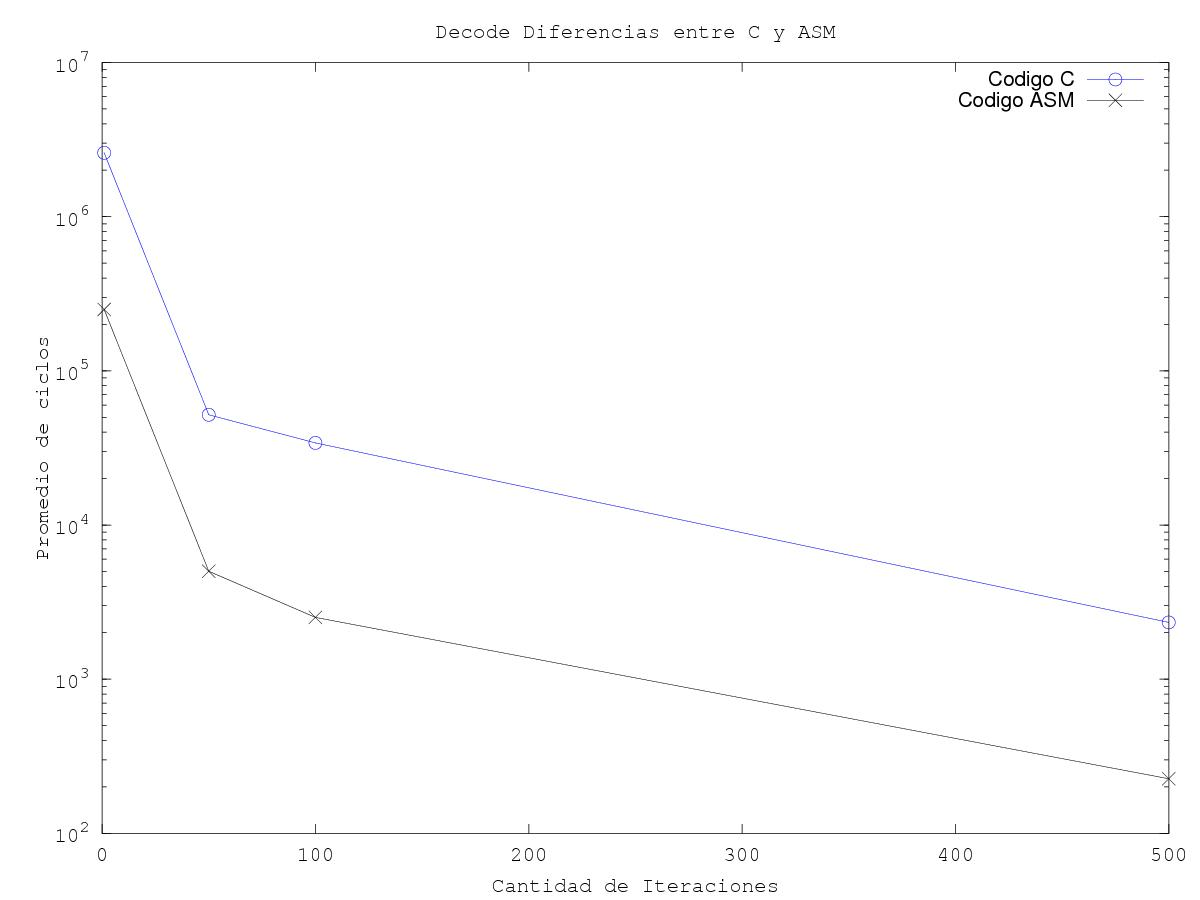
\includegraphics[scale=0.6]{imagenes/octave1.jpg}
\end{center}
\subsection{Resultados para experimentaci\'on variando n para distintas Fuerzas Máximas}
\subsubsection{Parametros de entrada Fijos:}
los parametros que no var\'ian son:
  \begin{itemize}
      \item span: 18
      \item h: 1
      \item $c_i$: 0.2
      \item Costo Unitario: 2000
      \item FMax: 0.5
  \end{itemize}
\subsubsection{Resultados segun n:}
  \begin{itemize}
   \item 
      \begin{itemize}
	\item n: 2
	\item Fuerza M\'axima resultante:F6 -1.83358
      \end{itemize}
   \item 
      \begin{itemize}
	\item n: 4
	\item Fuerza M\'axima resultante:F7 1.6
      \end{itemize}
   \item 
      \begin{itemize}
	\item n: 6
	\item Fuerza M\'axima resultante:F11 2.7
      \end{itemize}
   \item 
      \begin{itemize}
	\item n: 8
	\item Fuerza M\'axima resultante:F15 3.2
      \end{itemize}
   \item 
      \begin{itemize}
	\item n: 10
	\item Fuerza M\'axima resultante:F19 2.5
      \end{itemize}
   \item 
      \begin{itemize}
	\item n: 12
	\item Fuerza M\'axima resultante:F23 3.6
      \end{itemize}
   \item 
      \begin{itemize}
	\item n: 14
	\item Fuerza M\'axima resultante:F27 4.9
      \end{itemize}
   \item 
      \begin{itemize}
	\item n: 16
	\item Fuerza M\'axima resultante:F31 6.4
      \end{itemize}
   \item 
      \begin{itemize}
	\item n: 18
	\item Fuerza M\'axima resultante:F35 8.1
      \end{itemize}
  \end{itemize}
  \begin{center}
 \includegraphics[scale=0.6]{imagenes/octave2.jpg}
\end{center}
\subsection{Resultados para experimentaci\'on variando C para distintas Fuerzas Máximas}
\subsubsection{Parametros de entrada Fijos:}
los parametros que no var\'ian son:
  \begin{itemize}
      \item span: 18
      \item h: 1
      \item n: 6
      \item Costo Unitario: 2000
      \item FMax: 0.5
  \end{itemize}
\subsubsection{Resultados segun n:}
\begin{itemize}
    \item 
      \begin{itemize}
	\item $C_i$: 0.1
	\item Fuerza M\'axima resultante:F11 1.35
      \end{itemize}
    \item 
      \begin{itemize}
	\item $C_i$: 0.5
	\item Fuerza M\'axima resultante:F11 6.75
      \end{itemize}
    \item 
      \begin{itemize}
	\item $C_i$: 1
	\item Fuerza M\'axima resultante: F11 13.5
      \end{itemize}
    \item 
      \begin{itemize}
	\item $C_i$: 1.5
	\item Fuerza M\'axima resultante:F11 20.25
      \end{itemize}
    \item 
      \begin{itemize}
	\item $C_i$: 15
	\item Fuerza M\'axima resultante:F11 202.5
      \end{itemize}
\end{itemize}
  \begin{center}
 \includegraphics[scale=0.6]{imagenes/octave3.jpg}
\end{center}
\index{Resultado|)}
\index{Conclusiones|(}
\section{Conclusiones}

\subsection{Realizando cambio en los parametros se observa la variacion de la fuerza maxima ejercida:}

\begin{itemize}

\item \underline{Variando Span:} Sabemos por resultado que la fuerza m\'axima que se ha encontrado es una fuerza horizontal, sabemos que esta fuerza var\'ia dependiendo del valor span, esto se da porque al aumentar span, aumentan los valores de cosenos y disminuyen los de seno, y como coseno afecta a las fuerzas horizontales, la fuerza m\'axima aumenta. Caso inverso es si span disminuye.

\item \underline{Variando n:} ?`Por qu\'e ocurre que al aumentar n, en general aumentar la fuerza m\'axima?
Esto ocurre por que al aumentar el "n", hay mas cantidad de $C_i$ y entonces todas las dem\'as fuerzas se tensan m\'as y aumentan su fuerza en general.
Conclusi\'on: Si deseamos que la fuerza m\'axima de la estructura no sea muy grande, no es conveniente dividir en gran cantidad de $n$ el span. 

\item \underline{Variando $C_i$:} ?`Por qu\'e cuando aumenta $C_i$ aumenta la fuerza m\'axima y al disminuir $C_i$ disminuye la misma?
Esto se consigue porque si bien la fuerza m\'axima es horizonal y los $C_i$ interfiere en los links vertiles, los $C_i$ llegan tambi\'en a afectar los links horizontales. Esto se da por los links que est\'an colocados de forma hipotenusa, estos a trav\'es del seno y coseno le afectan y afecta a los links horizontales como verticales. Al aumentar el $C_i$, por la f\'ormula Fj*sen(o)+Fi+ci = 0 se observa que Fj y Fi se hacen m\'as chicos e incluso negativos, y si miramos el otro sector donde conecta el Fj, tendremos Fh-Fj*cos(o)-Fk = 0, siendo $Fk$ la fuerza m\'axima, como $Fj$ es negativo y disminuia su valor, -Fj*cos(o) sera positivo y da un valor m\'as grande que antes de recibir el aumento del $Ci$, por consiguiente $Fk$ va a tener que aumentar para que la igualdad se mantenga y por lo tanto aumentara su fuerza m\'axima.\newline
Mismo caso pero en sentido opuesto ocurrira si $C_i$ disminuye.


\end{itemize}

\subsection{Realizando cambio en los parametros para observar los cambios en el costo:}

\begin{itemize}

\item \underline{Variando n:} ?`Por qu\'e el valor n aumenta el costo?
Como ya dijimos al aumentar n se aumentan las fuerzas y por lo tanto se necesitar\'an m\'as pilares para reducirlas, adem\'as al aumentar n tendremos m\'as lugares en donde ubicar pilares. Esto \'ultimo mencionado nos sirve de mucha utilidad porque podremos poner muchos pilares lo que nos permitir\'ia construir una estructura mucho m\'as segura aunque el costo sea muy elevado.

\item \underline{Variando h:} ?`Por qu\'e al aumentar la altura disminuye la fuerza y al disminuirla aumenta?
Esto se da porque es exactamente lo opuesto al aumentar span, aca aumenta seno y disminuye coseno, a su vez esto afecta en la insercion de pilares, y en la fuerza m\'axima que soporta el puente.\newline
?`Conviene tener mucha o poca altura?
No conviene tener demasiada altura ni tampoco poca, ya que al variar la altura hay fuerzas que disminuyen y fuerzas que aumentan por lo tanto hay que tratar de encontrar el mejor equilibrio posible que nos permita tener el mejor ahorro en pilares.

\item \underline{Variando $F_{MAX}$:} ?`Por qu\'e al aumentar o disminuir el par\'ametro $F_{MAX}$, cambian los costos de la estructura?
Si aumentamos el par\'ametro $F_{MAX}$ lo que pasa es que estamos permitiendo que la estructura soporte hacer fuerzas demasiado grande y nos evitaremos construir pilares costoso. La desventaja de esto es que es probable que si la fuerza es muy grande los links se rompan haciendo que la estrictura del puente no sea segura y por lo tanto ocasionar accidentes. Si disminuimos dicho parametro es probable que se inserten mas cantidad de pilares y el puente sera mas costoso, pero tambien mas seguro.

\item \underline{Variando Span:} ?`Por que al aumentar span, aumenta el costo y viceversa?
Esto pasa porque al aumentar span, aumentamos la fuerza m\'axima, y por lo tanto llegar\'a m\'as rapido al rango $F_{MAX}$ y al superarlo se colocaran pilares en la estructura, aumentando el costo del mismo. Mismo caso si disminuimos el span, claro est\'a que el puente ser\'a m\'as corto.
Es importante destacar que si los cambios no son bruscos es probable que no sea necesaria la insercion de un pilar de m\'as.

\item \underline{Variando $C_i$:} ?'Por qu\'e al aumentar los valores de $C_i$ aumenta el costo y al disminuirlo ocurre lo opuesto?
Como sabemos por lo analizado y explicado en el punto 5.1, al aumentar $C_i$ aumentan las fuerzas y por lo tanto es m\'as probable utilizar m\'as cantidad de pilares para poder neutralizarlas. Esto como sabemos aumenta el costo de toda la estructura como se visualiza en los resultados.
\end{itemize}


\index{Conclusiones|)}
\index{Ap\'endices}
\section{Ap\'endices}

\index{Referencias}
\section{Referencias}
\begin{itemize}
\item R. Burden y J.D.Faires, An\'alisis num\'erico, International Thomson Editors, 1998.
\end{itemize}

\printindex

\end{document}
